\documentclass[12pt,a4paper]{article}

\usepackage[utf8]{inputenc}
\usepackage[T1]{fontenc}
\usepackage[spanish]{babel}
\usepackage{amsmath, amssymb}
\usepackage{graphicx}
\usepackage{float}
\usepackage{geometry}
\geometry{margin=2.5cm}
\usepackage{hyperref}
\usepackage{caption}
\usepackage{subcaption}
\usepackage{setspace}
\usepackage{titlesec}
\usepackage{siunitx}
\usepackage{xcolor} 
    \definecolor{codegreen}{rgb}{0,0.6,0}
    \definecolor{codegray}{rgb}{0.5,0.5,0.5}
    \definecolor{codepurple}{rgb}{0.58,0,0.82}
\usepackage{listings}
\renewcommand{\lstlistingname}{Anexo}


\onehalfspacing

% Para circuitos
\usepackage{circuitikz}

% Datos
\author{Nombre y Apellido \\ Legajo: XXXXX}
\date{\today}

\begin{document}

\setcounter{secnumdepth}{5}
\setcounter{tocdepth}{4}
\titleformat{\paragraph}[block]
  {\normalfont\normalsize\bfseries}
  {\theparagraph}                
  {1em}                            
  {}

      \lstdefinestyle{mystyle}{
    commentstyle=\color{codegreen},
    keywordstyle=\color{magenta},
    numberstyle=\tiny\color{codegray},
    stringstyle=\color{codepurple},
    basicstyle=\scriptsize\ttfamily, 
    breakatwhitespace=false,         
    breaklines=true,                 
    captionpos=b,                    
    keepspaces=true,                 
    numbers=left,                    
    numbersep=5pt,                   
    showspaces=false,                
    showstringspaces=false,
    showtabs=false,                  
    tabsize=2,
    frame=single,                  
    rulecolor=\color{black},
    title=\lstname               
}

\lstset{style=mystyle}

% Carátula personalizada
\begin{titlepage}
    \centering
    
\includegraphics[width=0.25\textwidth]{escudo.png} 
    \hspace{1cm}
    
\includegraphics[width=0.3\textwidth]{download.png} \\[1cm]

    {\large \textbf{UNIVERSIDAD NACIONAL DE CÓRDOBA} \\[0.5cm]}
    {\large \textbf {FACULTAD DE CIENCIAS EXACTAS, FÍSICAS Y NATURALES} \\[1cm]}
    {\Large SÍNTESIS DE REDES ACTIVAS \\[1cm]}

    \rule{\textwidth}{0.5pt} \\[0.5cm]
    {\Large \textbf{TP3 - Ejercicio Adicional} \\[0.3cm]}
    {\Large \textbf{Diseño de una Fuente de Tensión CC} \\[0.3cm]}
    \rule{\textwidth}{0.5pt} \\[1cm]

\begin{tabular}{l l}
\textbf{Profesor Titular:} & Dr. Ing. Ferreyra Pablo \\
\textbf{Profesor Adjunto:} & Ing. Reale Cesar \\
\\
\textbf{Alumnos:} & Dávila Tomassi, Carlos Valentino \\
 & Mendes Rosa, Agustín \\
 & Monja, Ernesto Joaquín \\
\end{tabular}\\[2cm]

{\centering
Año 2025
\par}

\end{titlepage}

% Índice
\tableofcontents
\newpage

\indent
\section{Motivación}

Si bien existen reguladores integrados ampliamente utilizados, el diseño de una fuente regulada discreta permite comprender en profundidad los principios de funcionamiento de los lazos de control, la regulación lineal y el impacto dinámico de las variaciones de carga sobre la estabilidad del sistema.

El presente trabajo aborda el diseño de una fuente de tensión continua de $5~[V]$, a partir de una fuente primaria de $12~[V]$ de $CC$. El objetivo no se limita únicamente a obtener el valor nominal de tensión requerido, sino también a garantizar una adecuada regulación frente a variaciones abruptas de carga, un rizado de salida acotado y un comportamiento dinámico estable.

\begin{figure}[H]
    \centering
    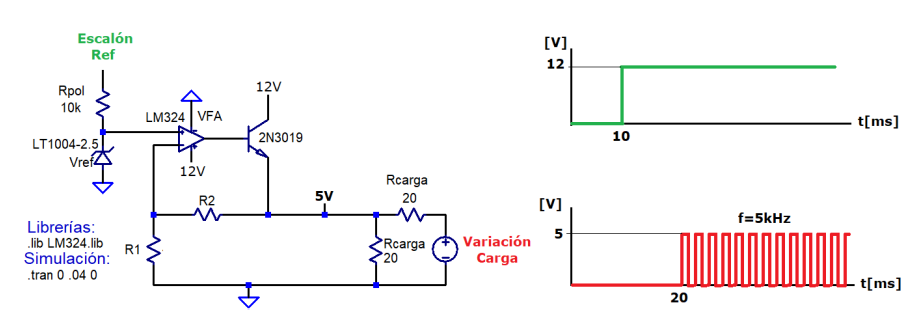
\includegraphics[width=1\linewidth]{Circuito.png}
    \caption{Fuente de Alimentación CC}
    \label{fig:placeholder}
\end{figure}

Se pide:
\begin{itemize}
    \item Agregar los componentes necesarios para alcanzar las especificaciones
    \item Simular el transitorio de los primeros $50~ms$, medir valor medio y ripple de estado estable
\end{itemize}

\newpage

\section{Marco Teórico}

\subsection{Fuentes de Alimentación Lineales:}

Una fuente de alimentación lineal es un sistema electrónico que proporciona una tensión continua regulada a partir de una fuente de mayor tensión, disipando el excedente de energía en forma de calor. A diferencia de las fuentes conmutadas, se caracterizan por su simplicidad y bajo nivel de ruido, a costa de una menor eficiencia energética.

En una fuente lineal regulada, la tensión de salida se busca mantener constante mediante un lazo de realimentación negativa que compara una fracción de la salida con una referencia de tensión estable. El error resultante es amplificado y controla un elemento activo, denominado elemento de paso, que regula la corriente suministrada a la carga.
\\

\subsection{Regulación por Realimentación:}

La regulación por realimentación negativa consiste en comparar la salida del sistema con un valor de referencia deseado. La diferencia entre ambos valores, conocida como señal de error, se amplifica y se utiliza para corregir la salida.

En el caso de una fuente regulada, la realimentación negativa permite:
\begin{itemize}
    \item Mantener constante la tensión de salida frente a cambios en la corriente demandada por la carga.
    \item Reducir la sensibilidad del sistema a variaciones de la tensión de alimentación primaria.
    \item Mejorar la estabilidad y el comportamiento dinámico del sistema, siempre que el lazo esté correctamente compensado.
\end{itemize}
\hspace{0.5 cm}

\subsection{Amplificador Operacional como Amplificador de Error:}

El amplificador operacional es un componente fundamental en el diseño de reguladores lineales discretos. En esta aplicación, se utiliza un LM324 para comparar la tensión de referencia con una fracción de la tensión de salida obtenida mediante un divisor resistivo.

Idealmente, el amplificador operacional presenta una ganancia infinita y una impedancia de entrada elevada, lo que permite que pequeñas variaciones en la tensión de error produzcan cambios significativos en su salida. En la práctica, la ganancia es finita y dependiente de la frecuencia, lo que introduce limitaciones en el ancho de banda y puede afectar la estabilidad del lazo de control.
\\

\subsection{Referencia de Tensión:}

Es el encargado de proporcionar un valor de tensión estable, independiente de las variaciones de la fuente de alimentación, la temperatura y la carga.

Su estabilidad permite mejorar la exactitud de la tensión regulada y reducir el error de salida, cualquier variación de la referencia se ve directamente reflejada en la tensión de salida del regulador.
\\

\subsection{Rizado de Tensión y Filtrado:}

El rizado de tensión (ripple) se define como la componente alterna superpuesta a la tensión continua de salida. En aplicaciones sensibles, el rizado debe mantenerse dentro de límites estrictos para evitar un funcionamiento incorrecto de los circuitos alimentados.

El uso de capacitores de desacople y filtrado en la salida del regulador permite reducir el rizado, almacenando energía y suministrándola a la carga durante variaciones rápidas de corriente. El valor del capacitor de salida se selecciona en función de la corriente máxima, la frecuencia de las perturbaciones y el rizado máximo admisible.
\\
\newpage
\section{Desarrollo}
\subsection{Análisis teórico y diseño:}

El circuito emplea una referencia de $2,5~[V]$ gracias a un regulador de tensión $TL431$, la cual constituye el punto de comparación del lazo de realimentación estando conectado a la entrada no inversora del amplificador operacional.

Por otro lado, en su entrada inversora el elemento es realimentado por una fracción de la tensión de salida obtenida mediante un divisor resistivo entre $R_1$ y $R_2$. De esta manera, la tensión realimentada es proporcional a la salida, según la expresión:

\begin{equation}
    \label{eq_1}
    V_f = V_o \left(\frac{R_1}{R_1 + R_2}\right)
\end{equation}
\hspace{0.5 cm}

Bajo condiciones ideales el amplificador operacional  opera de forma que la diferencia de potencial entre sus entradas tienda a cero, por lo que en estado estable debe cumplirse:

\begin{equation}
    \label{eq_2}
    V_f = V_{ref}
\end{equation}
\hspace{0.5 cm}

A partir de esta igualdad puede encontrarse la relación entre la tensión de referencia y la salida, imponiendo como condición el requerimiento de que la salida sea de $5~[V]$, y el valor de tensión de referencia ($2,5~[V]$), puede escribirse:

\begin{equation}
    \label{eq_3}
    V_{ref} = V_o \left(\frac{R_1}{R_1 + R_2}\right)
\end{equation}

\begin{equation}
    \label{eq_4}
    2,5 = 5 \left(\frac{R_1}{R_1 + R_2}\right)
\end{equation}
\hspace{0.5 cm}

Es posible moldear la ecuación (\ref{eq_4}) para despejar la relación entre resistencias, como se muestra a continuación:

\begin{equation}
    \label{eq_5}
    \left(1+\frac{R_2}{R_1}\right) = \frac{5}{2,5} 
\end{equation}

\begin{equation}
    \label{eq_6}
    \left(\frac{R_2}{R_1}\right) = 2-1 = 1 
\end{equation}
\hspace{0.5 cm}

Por lo tanto las resistencias del divisor deben ser iguales para cumplir las condiciones impuestas. Se elige un valor arbitrario de $R_1 = R_2 = 10~[k\Omega]$.
\\

\subsection{Primera simulación:}

A partir de los valores de resistencias obtenidos, se procedió a armar el circuito en el programa LTspice para simular su comportamiento y verificar que se cumplan los requerimientos. Se presenta a continuación el circuito utilizado para las pruebas:

\begin{figure}[H]
    \centering
    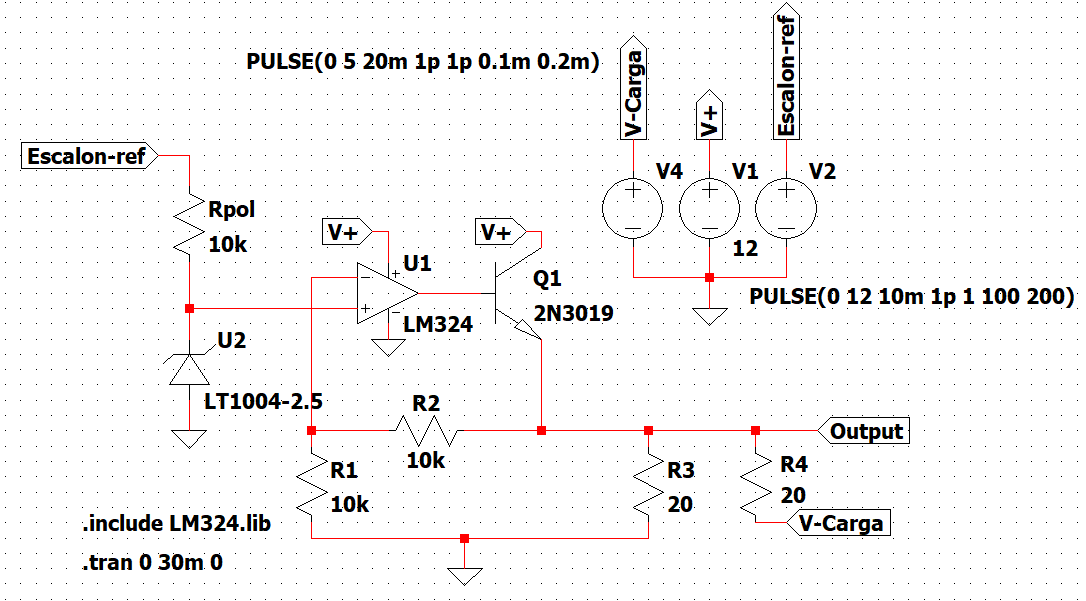
\includegraphics[width=1\linewidth]{Circuito_Spice.png}
    \caption{Diagrama circuital de la primera simulación}
    \label{fig:placeholder}
\end{figure}
\hspace{0.5 cm}

Se realizó un análisis temporal de $30~[ms]$ que permite ver el transitorio de los primeros instantes, se muestra a continuación:

\begin{figure}[H]
    \centering
    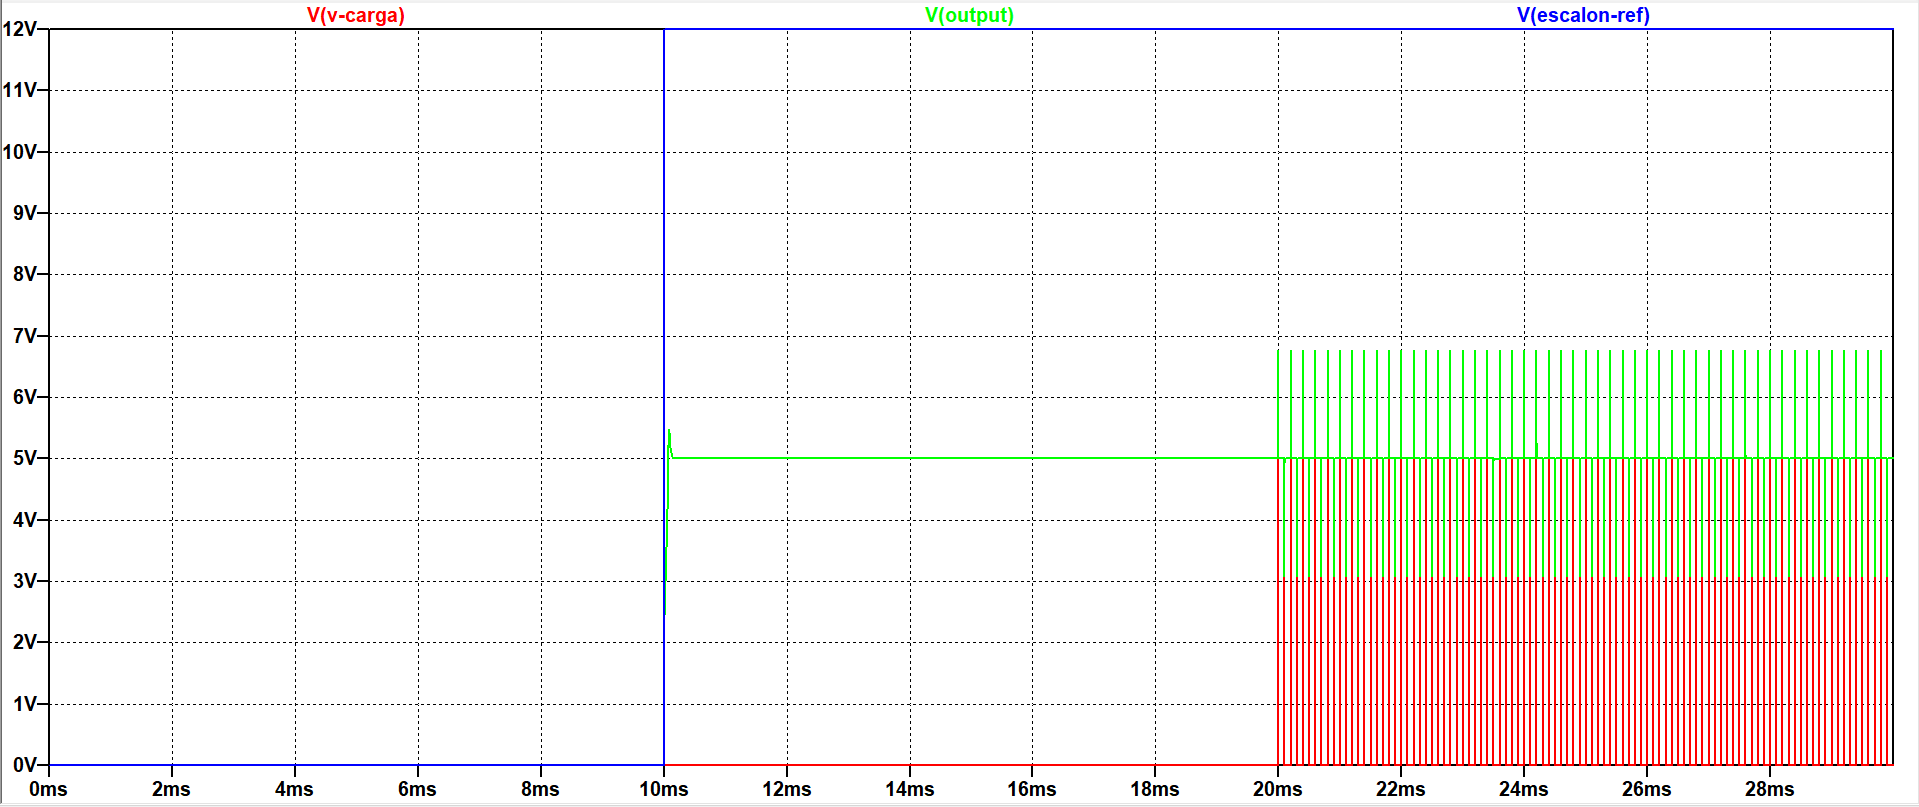
\includegraphics[width=1\linewidth]{TRAN_1.png}
    \caption{Transitorio de la primera simulación}
    \label{fig:placeholder}
\end{figure}

Se determina que mientras la carga se mantiene estable el sistema alcanza y mantiene los $5~[V]$, sin embargo con un sobrepasamiento de $0,5~[V]$ lo que queda por fuera de la tolerancia requerida. Además, al activar la variación de la carga, se tiene un rizado de:

\begin{equation}
    \label{eq_7}
    ripple_1 = \left(\frac{V_{max} - V_{min}}{V_{DC}}\right) = \left(\frac{6,8 - 3,2}{5}\right)100~\% = 72~\% 
\end{equation}
\hspace{0.5 cm}

Lo cual es un rizado sumamente excesivo para los requerimientos del sistema.

Se concluye que con el diagrama circuital que fue proporcionado no es suficiente solo valuar $R_1$ y $R_2$ para cumplir los requerimientos, ya que el nivel de rizado de este sistema es muy superior al objetivo y el nivel de sobrepico sobrepasa la tolerancia de $0,1~[V]$
\\

\subsection{Segunda simulación - Ajuste de Sobrepasamiento:}

El sobrepasamiento del sistema antes de estabilizarse en $5~[V]$ indica que está subamortiguado, es decir, que el lazo es muy rápido. Para esto se propone agregar un capacitor para agregar un polo que ralentice el sistema e impida o reduzca el sobrepasamiento.

El capacitor se coloca entre la salida y la entrada inversora del $LM324$. Se iteró su valor hasta que se cumpla el requerimiento de tolerancia, y el resultado se obtuvo con:

\begin{equation}
    \label{eq_8}
    C_c = 2,8~[nF]
\end{equation}
\hspace{0.5 cm}

Obteniendo así un sobrepasamiento de $0,04~[V]$, como se muestra en la siguiente figura:

\begin{figure}[H]
    \centering
    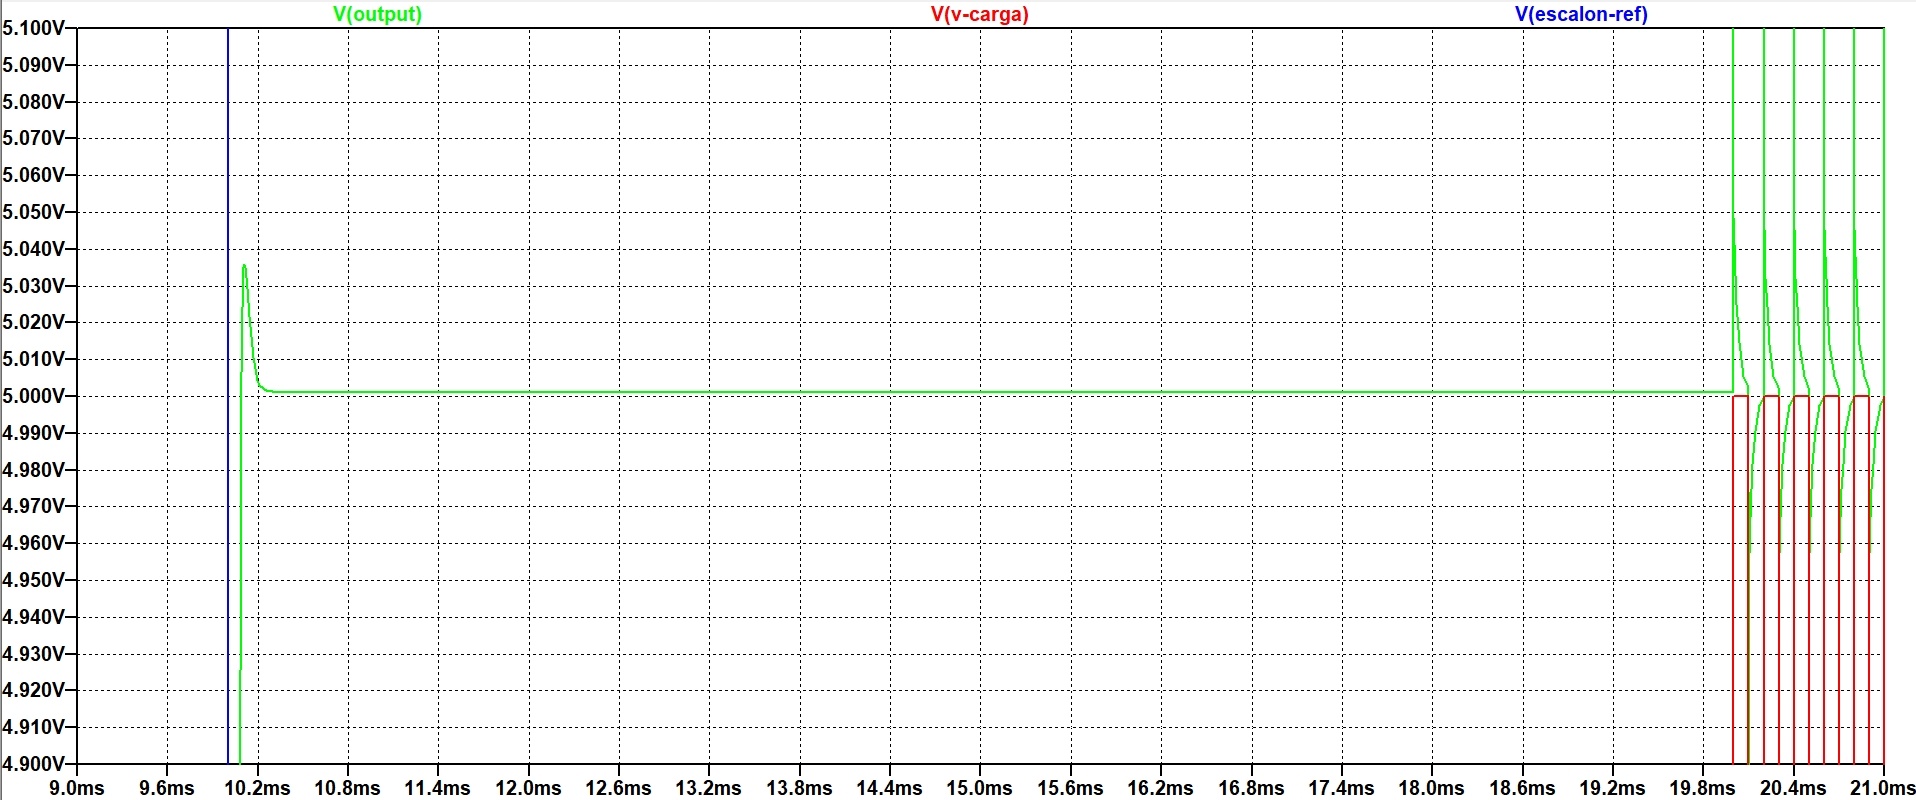
\includegraphics[width=1\linewidth]{Comp_Spice.png}
    \caption{Sistema con sobrepasamiento ajustado}
    \label{fig:placeholder}
\end{figure}

A continuación se muestra la disposición del circuito para la simulación anterior:

\begin{figure}[H]
    \centering
    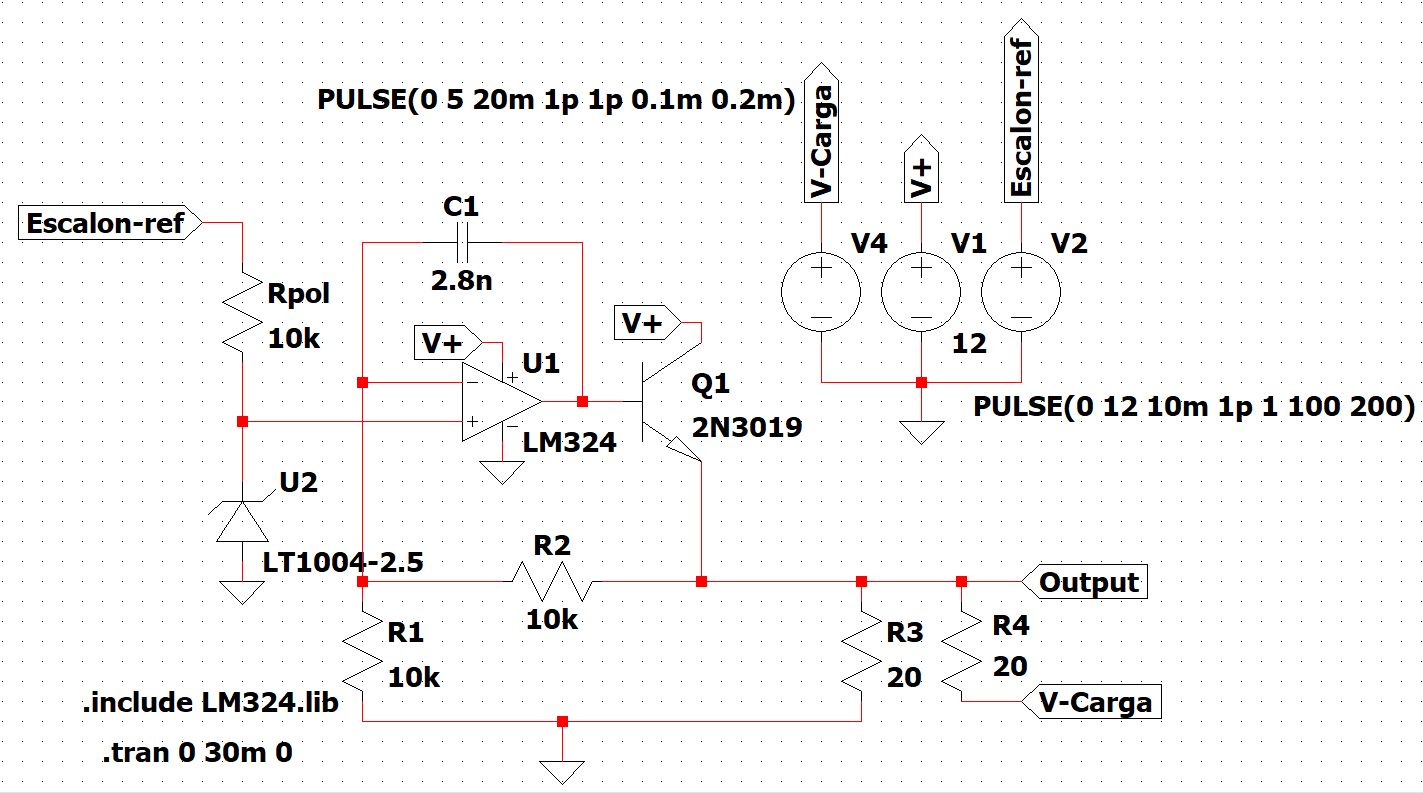
\includegraphics[width=1\linewidth]{Spice_Sobrepas.png}
    \caption{Diagrama circuital con capacitor de compensación}
    \label{fig:placeholder}
\end{figure}
\hspace{0.5 cm}

\subsection{Tercera simulación - Ajuste de Ripple:}

Debido al incumplimiento del objetivo de nivel de ripple, se procede a colocar un capacitor a la salida que absorba las variaciones rápidas de corriente que actualmente está pasando por el transistor entregando un ripple enorme.

El valor elegido luego de iterar fue de $470~[\mu F]$, el cual entrega el siguiente resultado:

\begin{figure}[H]
    \centering
    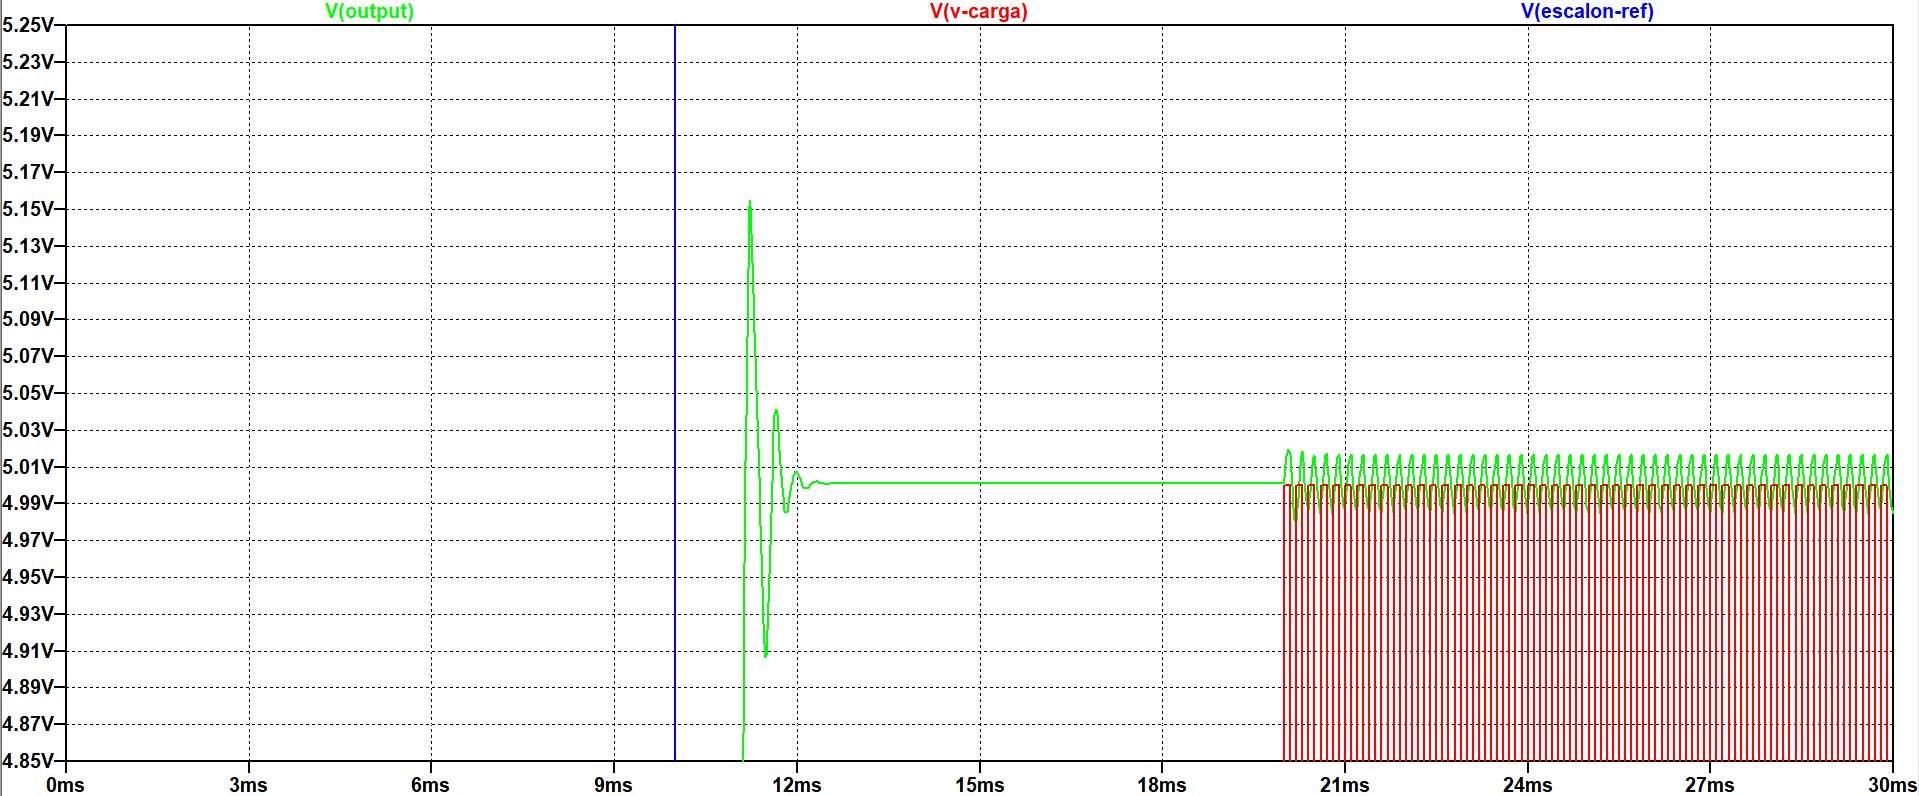
\includegraphics[width=1\linewidth]{TRAN_Ripple.png}
    \caption{Sistema con ripple ajustado}
    \label{fig:placeholder}
\end{figure}

Si bien el sistema cumple con la tolerancia de rizado, puede notarse que agregar el capacitor a la salida generó una oscilación en la respuesta del sistema al escalón, por lo tanto se volverá a modificar el capacitor de compensación, tal que se llegó a $C_c = 33~[nF]$, entregando el siguiente resultado:

\begin{figure}[H]
    \centering
    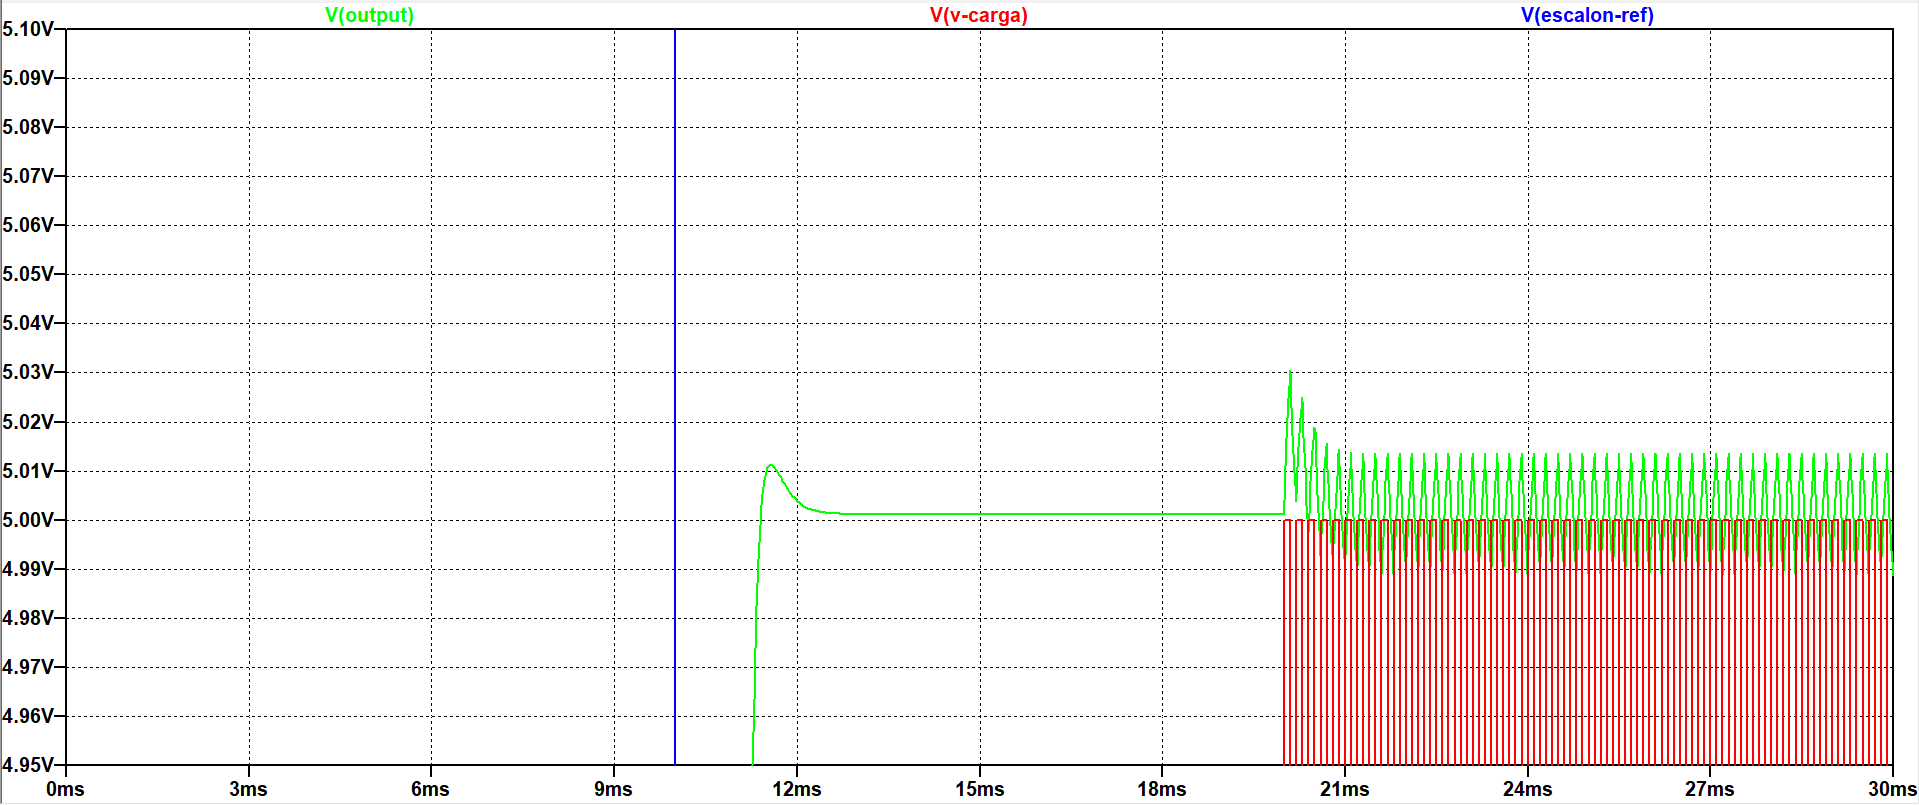
\includegraphics[width=1\linewidth]{TRAN_Final.png}
    \caption{Sistema con ajustes finales}
    \label{fig:placeholder}
\end{figure}

Finalmente, el ripple calculado para este circuito al variar la carga es de:

\begin{equation}
    \label{eq_9}
    ripple_3 = \left(\frac{5,014 - 4,988}{5}\right)100~\% = 0,52~\% 
\end{equation}
\hspace{0.5 cm}

Lo cual cumple con el requerimiento de que sea menor a $1\%$. Además, el sobrepasamiento es de $0,012~[V]$, lo cual se mantiene dentro de la tolerancia de tensión regulada.

A continuación se muestra la disposición del circuito para la simulación anterior:

\begin{figure}[H]
    \centering
    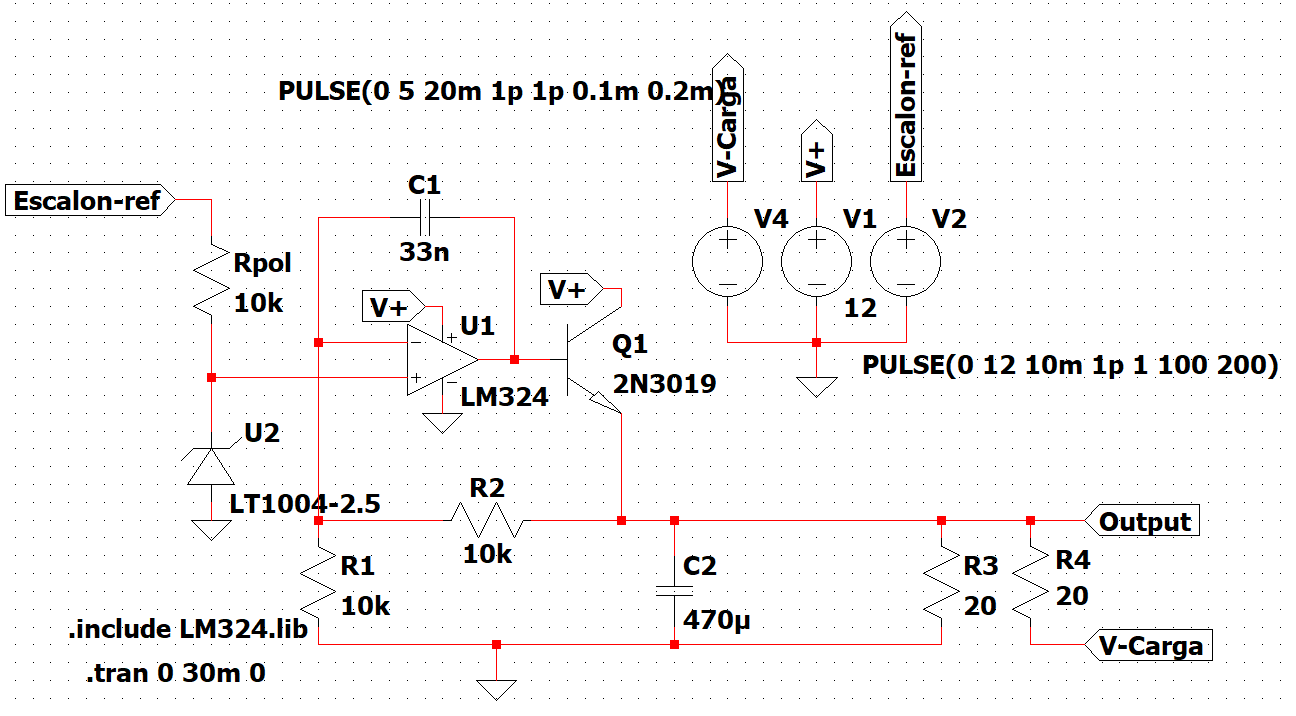
\includegraphics[width=1\linewidth]{Circ_Spice_Ripple.png}
    \caption{Diagrama circuital con capacitor de ripple}
    \label{fig:placeholder}
\end{figure}

\newpage
\section{Conclusiones}

En el presente trabajo se diseñó y analizó una fuente de tensión continua regulada de $5~[V]$ a partir de una fuente primaria de $12~[V]$, utilizando un regulador lineal discreto basado en realimentación negativa. El objetivo principal no fue únicamente obtener el valor nominal de tensión requerido, sino verificar el cumplimiento de las especificaciones dinámicas impuestas frente a variaciones de carga.

A partir del análisis teórico inicial se determinó la relación necesaria entre las resistencias del divisor de realimentación, estableciendo valores iguales entre ellas, lo que permitió alcanzar la tensión de salida deseada en régimen permanente. Sin embargo, las primeras simulaciones evidenciaron que el circuito original no cumplía con los requerimientos dinámicos, presentando un sobrepasamiento excesivo y un nivel de rizado inaceptable ante variaciones abruptas de carga.

Mediante el agregado de un capacitor de compensación se logró reducir el sobrepasamiento de la respuesta transitoria, asegurando que la tensión de salida permanezca dentro de la tolerancia especificada. Posteriormente, la incorporación de un capacitor de filtrado en la salida permitió reducir significativamente el rizado de tensión, cumpliendo con el requisito de un rizado menor al $1\%$. La interacción entre ambos elementos hizo necesario un ajuste final de la compensación para garantizar la estabilidad global del sistema.

Las simulaciones finales demostraron que el circuito cumple simultáneamente con los requerimientos de tensión regulada, bajo sobrepasamiento y bajo rizado, validando el diseño propuesto.

\end{document}